\section{Overview of Approach} \label{Sec:approach}
\IncMargin{0em}
\begin{algorithm}[t]
{\scriptsize
\SetKwInOut{Input}{input}\SetKwInOut{Output}{output}
\Input{Test suite $T$; The set of test cases $tc_i \in T$}
\Output{The ordered set of oracles $oracles$}
\BlankLine

\Begin {
\nl \For{$tc_i \in T$}{
\nl  $trace \leftarrow textsc{Exec}(tc_i)$\\
\nl  $domAccss \leftarrow \textsc{GetDOMAcc}(trace)$\\   	
\nl  $freqAccdDOM\leftarrow \emptyset$\\
\nl  \For{$dom \in domAccss $}{
\nl   \If{$\textsc{DOMUsgFreq}(dom) \geq \frac{1}{NoOfDOMElems} $}{
\nl    $freqAccdDOM \leftarrow dom \cup freqAccdDOM$\\       
      }
     }
\nl  \For{$asstn \in assertions_{tc_i}$}{
\nl   $asserDOMAcc \leftarrow \textsc{GetDOMAcc}(asstn)$\\
\nl   $asserDOMMuts \leftarrow \textsc{GetDOMMuts}(asserDOMAcc)$\\
\nl   \For{$domMut \in asserDOMMuts$}{
\nl    $bwSts \leftarrow \textsc{GetBWSlice}(domMut, trace)$\\
\nl    $asstnRel \leftarrow \textsc{GetWrVars}(bwSts)$\\
\nl    $potAsstnRel \leftarrow \textsc{GetFWSlice}(asstnRel, trace)$\\
      }
     }
\nl  $nonAsserDOMMuts \leftarrow \textsc{GetDOMMuts}(freqAccdDOM)$\\
\nl  \For{$domMut \in nonAsserDOMMuts$}{
\nl   $bwSts \leftarrow \textsc{GetBWSlice}(domMut, trace)$\\
\nl   $nonAsstnRel \leftarrow \textsc{GetWrVars}(bwSts)$\\
     }
\nl  $asstnRelOrcls[func]_{f=1}^{n} \leftarrow \textsc{GetValue}(\textsc{Accessibles}([func]_{f=1}^{n}, asstnRel))$\\
\nl  $candidOrcls[func]_{f=1}^{n} \leftarrow \textsc{Accessibles}([func]_{f=1}^{n}, [potAsstnRel \cup nonAsstnRel])$\\
\nl  $oracles[func]_{f=1}^{n}.\textsc{Add}(asstnRelOrcls \cup candidOrcls)$\\
   }
\nl $\textsc{Rank}(oracles[func]_{f=1}^{n})$\\
\nl return $(oracles[func]_{f=1}^{n})$
}
\caption{Oracle Generation} 
\label{Alg:algorithm}
}
\end{algorithm}
%\DecMargin{lem}
\begin{figure*}[!t]
  \centering
  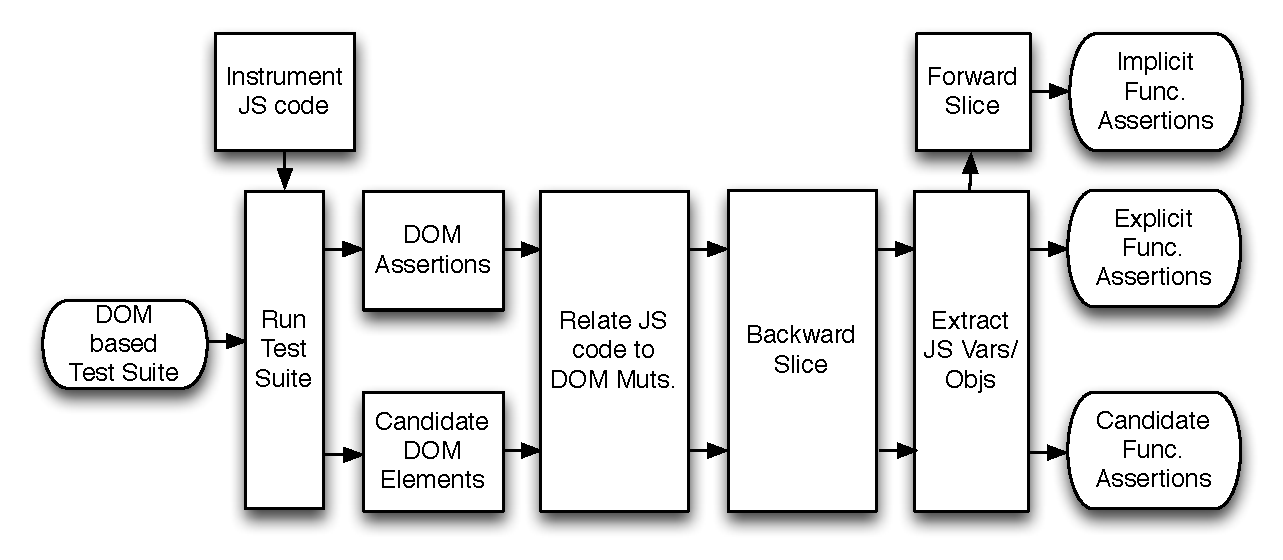
\includegraphics[width=.7\hsize]{fig/approachDiagram}
  \mycaption{Overview of our assertion generation approach.}
  \vspace{-0.1in} 
  \label{Fig:approachDiagram}
  \vspace{-0.1in} 
\end{figure*}
An overview of our \javascript function-level assertion generation technique is depicted \figref{approachDiagram}.
At high level, our approach generates function level assertions for the \javascript code by utilizing human written DOM-based tests and assertions. Our code level assertions fall in the following three categories: (1) explicit assertions, which are directly inferred from analyzing the manually written DOM-based assertions, (2) implicit assertions, which are indirectly affected by the human written DOM-based assertions, and (3) potential candidate assertions, which are not considered in the written DOM-based assertions, yet are potentially useful to be checked by the function level test suite. We describe our approach below. The numbers below in parentheses correspond to those in the boxes of \figref{approachDiagram}.

In the first part of our approach we (1) instrument the \javascript code and execute the instrumented application by running the existing DOM-based test suite. In this step we gather detailed execution trace of the application. We then extract (2) DOM assertions, which are DOM element accesses for each assertion, and (3) candidate DOM elements, which are useful DOM elements that can potentially be utilized for the purpose of assertion generation. We (4) identify the initial point of connection between the \javascript code and checked DOM element. We collect lines of code responsible for updating the corresponding DOM element. After determining DOM mutating statements, we (5) apply a backward slice on these statements to find the entire code blocks that update the checked DOM element. We (6) extract \javascript entities including variables and objects associated with each of the obtained statements. Accessible entities form our explicit function level assertions (7). We further (8) perform a forward slice on the extracted \javascript entities to identify statements, that are implicitly affected by such entities. The accessible \javascript variables/objects associated with collected statements form our implicit function level assertions (9). In addition to explicit and implicit assertions, which are either directly responsible for mutating checked DOM elements or indirectly affected by checked DOM elements, we also generate candidate assertions (10). Candidate assertions are involved with updating potentially useful DOM elements, which are not checked in the existing DOM-based assertions. To obtain candidate function level assertions, we perform step (4), (5), and (6) on the inferred candidate DOM elements (3).         
%mutation of customer.couponStatus = coupon.Id + '-' + 'used' to customer.couponStatus = coupon.Id + 'used';'